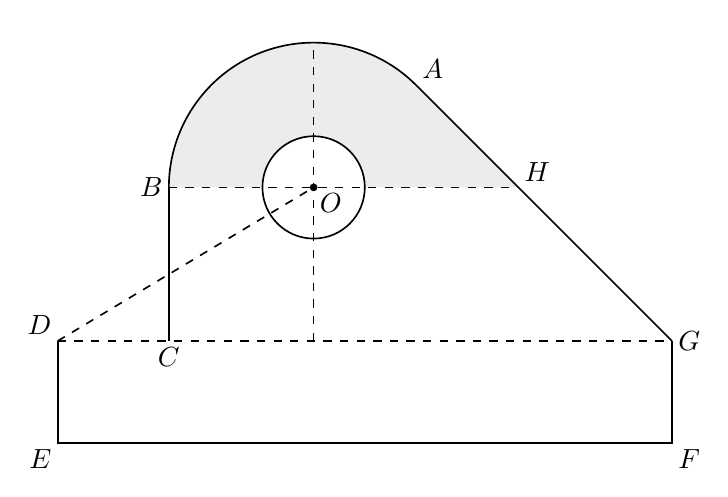
\begin{tikzpicture}[x=0.65cm,y=0.65cm,line width=.6pt,font=\normalsize]
\coordinate (D) at (0.000000000000,0.000000000000);
\coordinate (E) at (0.000000000000,-2.000000000000);
\coordinate (F) at (12.000000000000,-2.000000000000);
\coordinate (G) at (12.000000000000,0.000000000000);
\coordinate (O) at (5.000000000000,3.000000000000);
\coordinate (A) at (7.000000000000,5.000000000000);
\coordinate (B) at (2.171572875254,3.000000000000);
\coordinate (C) at (2.171572875254,0.000000000000);
\coordinate (M) at (5.000000000000,0.000000000000);
\coordinate (T) at (5.000000000000,5.828427124746);
\coordinate (H) at (9.000000000000,3.000000000000);
% Shade only the region ABOVE BH; lower BCGH is unshaded.
\fill[gray!15] (H)--(A) arc[start angle=45,end angle=180,radius=2.828427124746]--cycle;
\draw (A) arc[start angle=45,end angle=180,radius=2.828427124746];
\draw (B)--(C);\draw (A)--(G);\fill[white] (O) circle[radius=1];\draw (O) circle[radius=1];
\draw[dashed] (B)--(H);\draw[dashed] (D)--(G);\draw[dashed] (M)--(T);\draw[dashed] (D)--(O);\draw (D)--(E)--(F)--(G);
\fill (O) circle[radius=1.4pt];
\node[above left=2pt,inner sep=0pt] at (D) {$D$};
\node[below left=2pt,inner sep=0pt] at (E) {$E$};
\node[below right=2pt,inner sep=0pt] at (F) {$F$};
\node[right=2pt,inner sep=0pt] at (G) {$G$};
\node[left=2pt,inner sep=0pt] at (B) {$B$};
\node[below=2pt,inner sep=0pt] at (C) {$C$};
\node[above right=2pt,inner sep=0pt] at (A) {$A$};
\node[above right=2pt,inner sep=0pt] at (H) {$H$};
\node[below right=2pt,inner sep=0pt] at (O) {$O$};
\end{tikzpicture}
